\chapter{The Greensill Case}
\label{ch:greensill}

\section{Why Greensill}

Greensill Capital was a supply chain finance business founded in 2011 by Lex Greensill, an Australian former banker. By 2020 it was financing tens of billions of dollars of trade receivables, had attracted investment from SoftBank's Vision Fund, employed a former British prime minister as an adviser, and supplied the assets for a family of funds run by Credit Suisse that held about ten billion dollars of investors' money. In March 2021 it collapsed. Its trade credit insurance was not renewed, Credit Suisse froze its funds, the German regulator closed Greensill Bank in Bremen, and Greensill Capital's English companies entered administration. The fallout has occupied courts in England, Australia, Switzerland, Germany and the United States for five years.\index{Greensill Capital}

We use Greensill as a case study because it is a case about information. Investors relied on representations about the safety of the notes they bought. The notes were safe, it was said, because they were backed by receivables owed by creditworthy companies and insured against non payment. Insurers relied on representations about the risks they were insuring. Credit Suisse relied on Greensill's representations about the assets it originated. Each party had to form beliefs about default risk from information supplied by another, and each was later said to have been misled, or to have failed to ask the right questions. The doctrines of Chapters~\ref{ch:tort} and~\ref{ch:misrep}, epistemic responsibility, misrepresentation, inducement and the duty of fair presentation, were all engaged. Our tort paper used the case to show how those doctrines operate as Bayesian constraints \citep{polson_sokolov_tort}.

This chapter is not a narrative of the collapse, which has been told well by others, nor a judgment on contested allegations, many of which have never been tried. Where we describe events we rely on public statements, official reports and judgments; where matters are disputed we say so. Our aim is to show how a Bayesian analysis would frame the questions a court must answer.

\section{The business model}

\subsection{Supply chain finance}

In ordinary supply chain finance, also called reverse factoring, a large buyer arranges for a finance provider to pay its suppliers early, at a discount, and the buyer then pays the provider on the original due date. Suppliers get cash sooner; the buyer gets longer payment terms; the provider earns the discount. The credit risk is the risk that the buyer fails to pay, and since the buyer is typically a large, creditworthy company, the risk is low. The assets are short dated, typically ninety days or less, so the provider's exposure turns over quickly.\index{supply chain finance}

Greensill packaged such receivables into notes, which it sold to investors, principally the Credit Suisse supply chain finance funds. The funds marketed the notes as low risk, with the additional protection of trade credit insurance covering non payment by the obligors.

\subsection{Departures from the model}

As the business grew, it departed from the simple model in ways that matter for our analysis.

\paragraph{Concentration} A large share of Greensill's financing was extended to companies associated with a small number of clients, most notably the GFG Alliance group of companies controlled by Sanjeev Gupta. A diversified portfolio of receivables from many unrelated buyers has different risk from one in which a single group is a large share of the book.\index{GFG Alliance}

\paragraph{Future receivables} Greensill financed what it called prospective or future receivables: amounts that it expected to be owed in the future by companies that might buy from the client, rather than invoices for goods already delivered. These were in substance unsecured loans to the client, repayable from the client's future sales. The credit risk was the client's, not that of established buyers. In litigation brought by the coal company Bluestone Resources against Greensill in the federal court in New York, Bluestone alleged fraud and that Greensill had financed it on the strength of its long-term prospects rather than on existing receivables.

\paragraph{Insurance} The trade credit insurance was written largely through Bond and Credit Company, an Australian underwriter acquired by Tokio Marine in 2019, and its terms and the conduct of the underwriter became the subject of dispute. When the insurers declined to renew policies that expired at the start of March 2021, Greensill sought a mandatory injunction in the Supreme Court of New South Wales to compel Insurance Australia to renew two policies; the court refused the application on 1 March 2021. Without insurance the notes could not be sold, and the business stopped.

\paragraph{Related lending} The Credit Suisse funds lent money to companies in which SoftBank, an investor in Greensill, also held stakes, among them the construction company Katerra. Credit Suisse funds later sued SoftBank in the High Court in London over a 440 million dollar payment in November 2020, and lost (\emph{[2025] EWHC 2631 (Ch)}); the court found SoftBank had acted in good faith.

\begin{figure}[t]
\centering
\begin{tikzpicture}[node distance=1.2cm and 1.6cm, every node/.style={font=\scriptsize},
 box/.style={rectangle, rounded corners, draw=nightblue, fill=softgray, align=center, minimum width=2cm, inner sep=3pt},
 ar/.style={-{Stealth[length=1.6mm]}, nightblue}]
\node[box] (inv) {Investors in\\ Credit Suisse funds};
\node[box, right=of inv] (cs) {Credit Suisse\\ SCF funds};
\node[box, right=of cs] (gc) {Greensill\\ Capital};
\node[box, below=of gc] (cl) {Clients\\ (e.g. GFG, Bluestone)};
\node[box, below=of cs] (ins) {Trade credit\\ insurers};
\node[box, below=of inv] (ob) {Obligors\\ (actual or prospective)};
\draw[ar] (inv) -- node[above] {cash} (cs);
\draw[ar] (cs) -- node[above] {buys notes} (gc);
\draw[ar] (gc) -- node[right] {advances} (cl);
\draw[ar] (ob) -- node[above] {pay receivables} (cl);
\draw[ar] (ins) -- node[right] {cover} (cs);
\draw[ar, dashed] (gc) -- node[above, sloped] {presentation of risk} (ins);
\draw[ar, dashed] (gc.north) to[bend right=25] node[above] {representations about assets} (cs.north);
\end{tikzpicture}
\caption{The flows of money and of representations in the Greensill structure. Solid arrows carry money or cover; dashed arrows carry information on which other parties relied.}
\label{fig:greensillflows}
\end{figure}

\section{The chain of beliefs}

Figure~\ref{fig:greensillflows} shows the structure. Money flowed from investors through the funds to Greensill and its clients, and was supposed to flow back from obligors. Information flowed in the other direction. Investors relied on the funds' descriptions of the assets; the funds relied on Greensill's origination and on the insurance; the insurers relied on Greensill's presentation of the risks. At each link a party formed a posterior on default risk using information supplied by the next party along.

In Bayesian terms, each link is a channel with a likelihood, and information can only be lost, never gained, as it passes along the chain. Let $\theta$ denote the true default risk of the portfolio and $s_k$ the signal passed at link $k$. The investor's posterior depends on the composition of the channels,
\begin{equation}
\Prob(\theta\given s_1) \propto \Prob(\theta) \int\!\!\int \Prob(s_1\given s_2)\Prob(s_2\given s_3)\Prob(s_3\given \theta)\,ds_2\,ds_3,
\end{equation}
and the informativeness of $s_1$ about $\theta$ can be no greater than that of the least informative link, by the data processing inequality. A chain of trust is only as strong as its weakest link. If the insurer's assessment depended on an underwriter who was not independent, or if the funds' due diligence on assets relied on the originator's own descriptions, then the investor's apparently strong signal of safety, insured notes in a bank sponsored fund, carried much less information about $\theta$ than it appeared to.\index{data processing inequality}

\section{Concentration and tail risk}

The first quantitative question is what concentration does to the distribution of losses. Figure~\ref{fig:greensillloss} compares two simulated portfolios. In the first, two hundred obligors each represent half a per cent of the book, with an annual default probability of three per cent and a moderate default correlation. In the second, one obligor represents half the book and the other half is spread over one hundred and ninety nine obligors. The expected loss is the same in both. The tail is completely different. The concentrated portfolio has a roughly three per cent chance of losing half the fund in a year; the diversified one does so with a probability of about two in a hundred thousand.\index{concentration risk}

\begin{figure}[t]
\centering
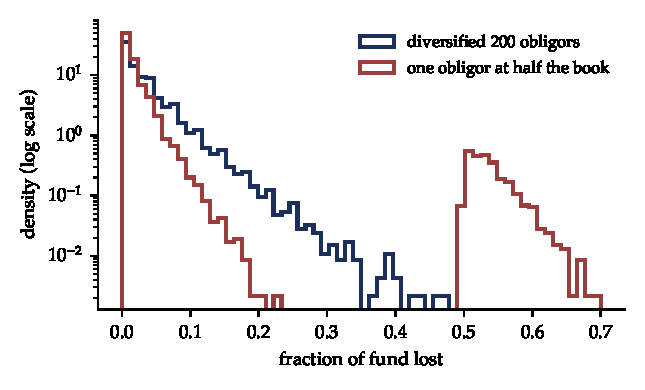
\includegraphics[width=\linewidth]{fig_greensill_loss}
\caption{Simulated distribution of annual losses for a diversified receivables portfolio and for one in which a single obligor accounts for half the book. Both have the same expected loss. Simulation with a one factor Gaussian copula, default probability three per cent and asset correlation $0.2$.}
\label{fig:greensillloss}
\end{figure}

The legal significance is that expected loss, the figure most easily stated, is not the figure an investor in a low risk fund cares about. A representation that a fund holds short dated, insured receivables of investment grade obligors conveys a belief about the whole distribution, in particular that the probability of a large loss is negligible. If the actual portfolio was concentrated, that implied belief was false even if the expected loss was correctly stated. This is a half truth in the sense of \emph{Dimmock v Hallett} \citep{dimmock1866}: the statement is literally consistent with the facts but conveys a posterior the speaker's information does not warrant.

\section{Future receivables as a change of hypothesis}

The second question concerns future receivables. A receivable is a claim on a buyer that has bought goods and promised to pay. A future receivable is an expectation that some buyer will do so. The default probability of a pool of existing receivables from large buyers is low because those buyers are creditworthy and have already incurred the obligation. The default probability of a loan repayable from future sales depends on whether the sales happen, which depends on the client's business, and on whether the proceeds reach the lender.

In the language of Chapter~\ref{ch:bf}, a pool of future receivables is a different hypothesis from a pool of existing receivables, with a different likelihood for repayment. Describing the former as the latter is not a small misstatement of a parameter but a misstatement of the model. The Kullback Leibler measure of Chapter~\ref{ch:misrep} makes this concrete. If the warranted probability of a large loss on a future receivables loan to a weak client is ten per cent and the conveyed probability is one tenth of one per cent, the divergence $D(p\,\|\,q)$ is about $0.37$ nats, nine times the mild overstatement of Chapter~\ref{ch:misrep} (about $0.04$ nats) though well short of its gross one (about $1.6$ nats).

\section{Updating on payment history}

The third question is what a lender or investor monitoring the portfolio should have inferred from its performance. Suppose an obligor's payments are observed over time and some are late or rolled over. A simple model treats each settlement as a Bernoulli trial with probability $\phi$ of difficulty. With a beta prior reflecting an initially favourable view, say $\text{Beta}(1,30)$ with mean about three per cent, a record of two late settlements in twelve moves the posterior mean to about seven per cent; six in twenty four moves it to about thirteen per cent (Figure~\ref{fig:greensillbeta}).

\begin{figure}[t]
\centering
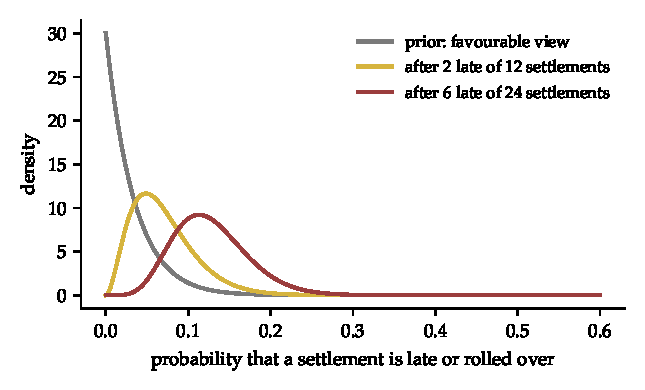
\includegraphics[width=\linewidth]{fig_greensill_beta}
\caption{Posterior distributions for the probability that an obligor's settlement is late or rolled over, as late or rolled settlements accumulate, starting from a favourable prior. Illustrative.}
\label{fig:greensillbeta}
\end{figure}

When a lender rolls over maturing receivables rather than collecting them, as can happen when a client cannot pay and the lender refinances, the observed record of defaults is censored: problems are concealed by refinancing. A Bayesian monitor should treat rollovers as partial evidence of distress, not as clean repayments. Investigations of Credit Suisse's handling of its Greensill relationship, including the Swiss regulator's 2023 finding that the bank had seriously breached its supervisory obligations \citep{finma2023}, describe internal warnings that were not acted on. The general lesson is that an institution's risk system should update on adverse signals, and that failure to update when the evidence warrants is a failure of epistemic responsibility.\index{Credit Suisse}\index{FINMA}

\section{The insurance questions}

The insurers' position in the litigation that followed was, in broad terms, that the policies were not valid or did not respond, because of non disclosure and other defences. Greensill and the Credit Suisse funds contended otherwise. Many of the principal claims were brought in the Federal Court of Australia. A large claim by Credit Suisse funds against the insurer Insurance Australia was reported settled before trial, in 2026 according to trade press reports. We do not express any view on the merits.

What the Bayesian framework offers is a way to organise the questions such a case raises, using the English law of fair presentation as the template.
\begin{enumerate}[label=(\alph*)]
\item What did the insured know or ought to have known about the risk, $D_S$ in the notation of Chapter~\ref{ch:misrep}?
\item Was that information presented fairly, so that a prudent insurer's posterior on loss would have been what $D_S$ warranted?
\item If not, what posterior would a prudent insurer have formed with a fair presentation, and what decision, premium or terms would it have made?
\item Was any failure deliberate or reckless, in which case the remedy is avoidance, or merely careless, in which case the remedy depends on what the insurer would have done?
\end{enumerate}
Question (c) is a counterfactual. It requires a model of the insurer's underwriting: how it priced risk as a function of concentration, obligor quality and the nature of receivables. The insurer's own underwriting guidelines, pricing models and correspondence are the evidence. A court applying the Insurance Act 2015 would ask the insurer to show the premium it would have charged, and would reduce the claim in proportion. This is an expected utility comparison of the kind Lindley advocated for courts \citep{lindley1991}.

There is a further layer. If the insurer's own underwriter had a relationship with the insured that compromised his independence, the insurer's posterior was formed through a corrupted channel. Whether the insured can rely on cover written by an agent who exceeded his authority, and whether the insurer is bound by what its agent knew, are questions of agency law. In Bayesian terms they ask whose information set defines the insurer's knowledge.

\section{The directors' responsibility}

In June 2026 the Insolvency Service announced that Lex Greensill had given a disqualification undertaking under which he may not act as a director of a company in the United Kingdom for nine years. The undertaking was given days before a six week trial of the Secretary of State's claim, which had sought a longer period; Greensill had earlier failed in an application to strike out the proceedings. An undertaking involves the director not disputing certain facts for the purposes of the disqualification proceedings only. The Insolvency Service's statement said, among other things, that he had caused Greensill companies to enter transactions in late 2020 that removed legal protections underpinning a Credit Suisse fund's investment.\index{director disqualification}

The Company Directors Disqualification Act 1986 requires the court to disqualify a director of an insolvent company whose conduct makes him unfit to be concerned in the management of a company. Unfitness is assessed on the civil standard, but the seriousness of the consequences has led courts to examine the evidence with care. In the language of Chapter~\ref{ch:standards}, the standard is a posterior threshold of one half, and the care reflects a low prior for the most serious allegations rather than a higher threshold. A disqualification undertaking is a settlement: the parties agree on a period in light of their posteriors about the likely outcome of trial and its costs, a subject we model in Chapter~\ref{ch:becker}.

\section{Political access and the value of information}

Greensill's lobbying of government ministers in 2020, on behalf of the company's access to emergency lending schemes, through the former prime minister David Cameron, led to a parliamentary inquiry and a government review. The House of Commons Treasury Committee concluded in 2021 that there had been a significant lack of judgment in the way the former prime minister lobbied, though it found no breach of the lobbying rules as then drafted \citep{treasury2021}. The episode is relevant here for a narrow reason. Access to decision makers is valuable because it lets a party supply information, and selected information, to someone whose decision affects it. The theory of Bayesian persuasion in Chapter~\ref{ch:misrep} applies: a sender who controls the information structure can move a receiver's posterior in its favour without stating a falsehood. Rules on lobbying are, in part, rules about which information structures are permitted.

\section{A Bayesian network for the case}

Figure~\ref{fig:greensillbn} is a simplified Bayesian network for the core inferential questions. The latent variables are the true quality of the asset pool, $Q$, the client concentration, $C$, and whether receivables were existing or prospective, $R$. These determine the default risk $\theta$. The signals are the fund documentation, the insurance cover, and the observed payment history. The insurer's decision to write cover depends on its posterior on $\theta$, which in turn depends on what was presented. The network makes explicit that the presence of insurance is not independent evidence of low risk if the insurance decision was itself based on the same, possibly incomplete, information. Treating the insurance as an additional, independent safety signal double counts.\index{double counting}

\begin{figure}[t]
\centering
\begin{tikzpicture}[node distance=1.0cm and 1.3cm, every node/.style={font=\scriptsize},
 lat/.style={circle, draw=nightblue, fill=softgray, minimum size=8mm, inner sep=1pt},
 obs/.style={rectangle, draw=nightblue, fill=starlight!30, minimum size=7mm, inner sep=2pt, align=center},
 ar/.style={-{Stealth[length=1.6mm]}, nightblue}]
\node[lat] (Q) {$Q$};
\node[lat, right=of Q] (C) {$C$};
\node[lat, right=of C] (R) {$R$};
\node[lat, below=of C] (th) {$\theta$};
\node[obs, below left=1.0cm and 0.6cm of th] (doc) {fund\\ documents};
\node[obs, below=1.0cm of th] (ins) {insurance\\ cover};
\node[obs, below right=1.0cm and 0.6cm of th] (pay) {payment\\ history};
\node[obs, left=1.6cm of th] (pres) {presentation\\ to insurer};
\draw[ar] (Q) -- (th); \draw[ar] (C) -- (th); \draw[ar] (R) -- (th);
\draw[ar] (th) -- (pay);
\draw[ar] (Q) -- (pres); \draw[ar] (C) to[bend right=35] (pres);
\draw[ar] (pres) -- (ins);
\draw[ar] (pres) -- (doc);
\draw[ar] (ins) -- (doc);
\end{tikzpicture}
\caption{A simplified Bayesian network for the Greensill inference problem. The insurance cover depends on the presentation, not directly on the true risk, so it is not an independent signal of low risk.}
\label{fig:greensillbn}
\end{figure}

\section{Loss and causation}

If a court were to find that investors were induced by misrepresentation to buy notes, it would need to assess loss. The measure in deceit, and under section 2(1) of the Misrepresentation Act 1967, is the loss flowing from entering the transaction, comparing the investor's position with where it would have been had it not invested. In negligent misstatement, after the Supreme Court's decision in \emph{Manchester Building Society v Grant Thornton}, the court asks about the scope of the duty: what risk the adviser was responsible for guarding against, and whether the loss falls within it \citep{mbs2021}. In Bayesian terms, scope of duty asks which component of the investor's posterior the defendant undertook to get right. A fund manager who undertook to describe the composition of the portfolio is responsible for losses that flow from its concentration; an insurer responsible only for paying claims under the policy is not responsible for losses from uninsured risks.

Proportionality arises again. Suppose investors would have invested in a fund correctly described as holding concentrated and partly prospective receivables, but at a higher yield. The loss attributable to the misrepresentation would then be, on a Bayesian view, not the whole loss but the difference between the outcome and what they would have accepted at a fair price. This is the counterfactual decision analysis of the Insurance Act applied to investment: the remedy should reflect the decision the claimant would have made with a correct posterior.

\section{Lessons}

Greensill teaches four lessons that recur in this book.

First, chains of reliance weaken information. Each additional party that passes on another's assessment adds noise and possibly bias, and the final recipient's posterior should reflect the weakest link. Legal doctrines of reliance and scope of duty allocate responsibility along such chains.

Second, the shape of the loss distribution matters as much as its mean. Representations about safety are representations about tails. The law of misrepresentation should judge them by what they imply about the probability of large losses, not only expected losses.

Third, signals that are not independent should not be added. Insurance written on the originator's presentation is not an independent check on the originator. Courts and regulators should ask what each signal adds given the others.

Fourth, the Bayesian remedy is counterfactual and proportional. English insurance law has adopted it. The law of misrepresentation in investment would benefit from doing the same. Chapter~\ref{ch:bankruptcy} turns to the bankruptcy courts, where the same questions about what was knowable at the time of a transaction arise in a different form.

\section*{Notes and Questions}
\addcontentsline{toc}{section}{Notes and Questions}
\begin{enumerate}[label=\arabic*.]
\item Using a one factor Gaussian copula, compute the probability that a portfolio with one obligor at fifty per cent of the book loses more than forty per cent in a year, for default probabilities of one, three and five per cent. Comment on the sensitivity.
\item Write a short representation that a fund manager might make about a supply chain finance fund. Identify the implied beliefs about the loss distribution. Which facts about the portfolio would make the representation a half truth?
\item In the beta model of this chapter, how many on time settlements would be needed after six late settlements in twenty four to bring the posterior mean back below five per cent?
\item An insurer charged $0.4$ per cent for cover; a fair presentation would have led it to charge $1.2$ per cent. A claim of fifty million pounds is made. What does the insurer pay under Schedule 1 of the Insurance Act 2015 if the breach was careless? If it was reckless?
\item Explain, using the network in Figure~\ref{fig:greensillbn}, why the presence of insurance should not be treated as independent evidence of low risk by an investor. When could it be?
\item Read the Insolvency Service's statement of June 2026 on the disqualification undertaking. Which of the facts stated bear on epistemic responsibility and which on decision responsibility?
\end{enumerate}

\section*{Further reading}
Our tort paper uses Greensill as its main example \citep{polson_sokolov_tort}. The House of Commons Treasury Committee report \emph{Lessons from Greensill Capital} (2021) and the Swiss regulator's 2023 statement on Credit Suisse are the main official accounts \citep{treasury2021,finma2023}.
